\thumbchapter{Einleitung}

Dies ist eine Vorlage für Abschlussarbeiten. Der Typ der Arbeit und die betreuenden Professoren sowie das Thema müssen in \path{titlepage.tex} geändert werden. Zusätzliche Kapitel und Verzeichnisse werden in \path{Master_Thesis.tex} eingefügt. Dabei sollte eine neue \path{.tex} Datei für die einzelnen Kapitel verwendet werden, da dadurch die Arbeit übersichtlicher wird.

Das Seitenlayout (Ränder, Daumenregister, Papierformat, ...) ist in \path{packages.tex} definiert und kann dort angepasst werden. Näheres dazu in den Kommentaren dieser Datei.

Der Abstract wird in \path{abstract.tex} angepasst und der Anhang befindet sich in \path{anhang.tex}.

\begin{align}
	\text{grad}(L_\pi) &= \frac{\partial L_\pi}{\partial \omega_{ij}} \\
	\hat{m_t} &= \frac{1}{1-{\beta_1}^t} \left[ \beta_1 m_{t-1} + (1 - \beta_1) \text{grad}(L_\pi) \right] \\
	\hat{v_t} &= \frac{1}{1-{\beta_2}^t} \left[ \beta_2 v_{t-1} + (1 - \beta_2) (\text{grad}(L_\pi))^2 \right]
\end{align}

\begin{align}
	L_\pi &= \frac{1}{N_E} \sum_{E} {L_\pi}_E
\end{align}

\begin{align}
	\Delta \omega_{ij} &= - \alpha \frac{\hat{m_t}}{\sqrt{\hat{v_t}} + \epsilon} 
\end{align}

\begin{align}
	\beta_1 &= 0,9 \\
	\beta_2 &= 0,999
\end{align}

\begin{align}
	y_i &= \max \left( 0; ~\sum_j \omega_{ij} \cdot x_j \right)
\end{align}

\begin{align}
	g_i(\xi, \boldsymbol{\omega}^i, \mathbf{x}^i) &= P \left\{ y_i = \xi | s_i \right\} \\
	s_i &= \sum_j \omega_{ij} \cdot x_j
\end{align}


\section{Beispiele}

Für Formeln verwendet man \lstinline|\begin{align}|.
	
\begin{align}
	e^{i \pi} &= -1 \\
	e &= \sum_{k=0}^{\infty}\frac{1}{k!}
\end{align}

Für nicht numerierte Formeln wird der Befehl \lstinline|\notag| verwendet.
\\
\autoref{diesIstEinLabel} ist ein Beispiel für ein eingebundenes Bild:

\begin{figure}[H] % H steht für "an dieser Stelle", "h" steht für "möglichst an dieser Stelle".
	\centering
	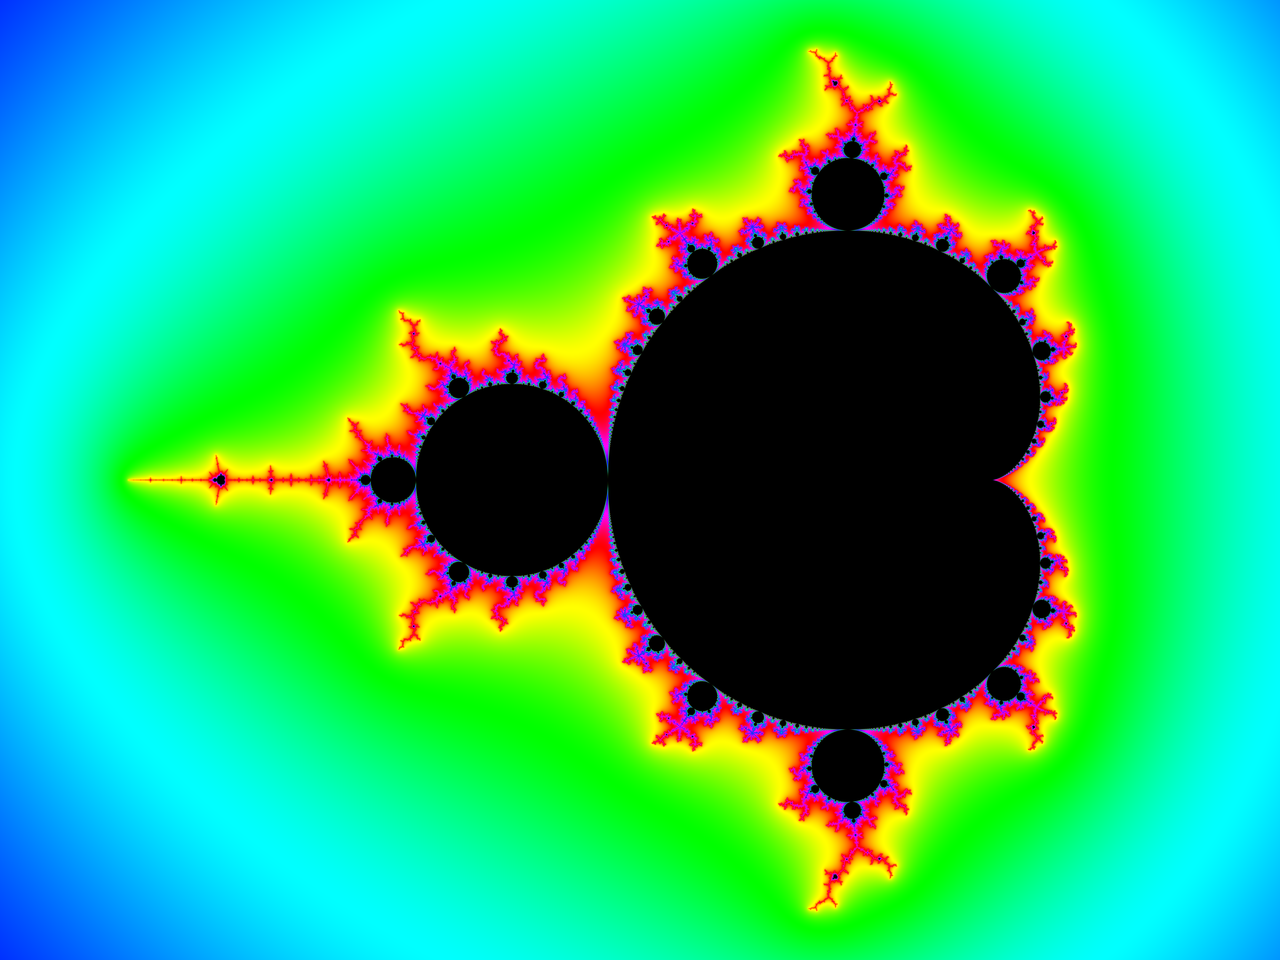
\includegraphics[width=.8\linewidth]{Bilder/mandelbrot}
	\bildquelle{Geek3, CC BY 3.0, \url{https://w.wiki/33UD}}
	\caption{Mandelbrot Rendering}
	\label{diesIstEinLabel} % Wichtig: Labels müssen immer UNTER dem Caption stehen!
\end{figure}

% Tipp für Wiki Quellen: https://meta.wikimedia.org/wiki/Special:UrlShortener


Mehrere Bilder in einer Abbildung sind auch möglich:

\begin{figure}[H]
	\centering
	\subfloat[Vogel\label{bild1}]{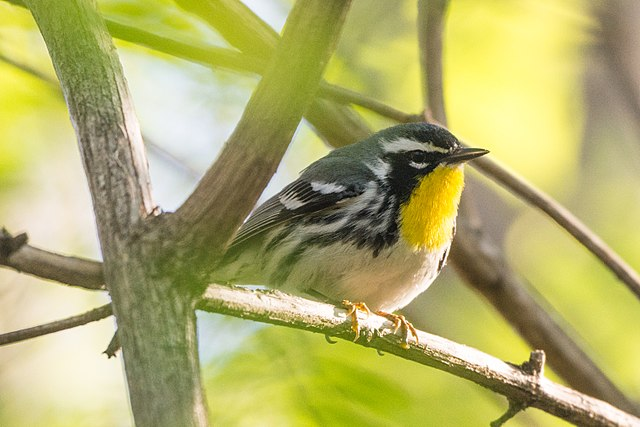
\includegraphics[width=0.45\linewidth]{Bilder/vogel}}%
	\qquad
	\subfloat[Kuh\label{bild2}]{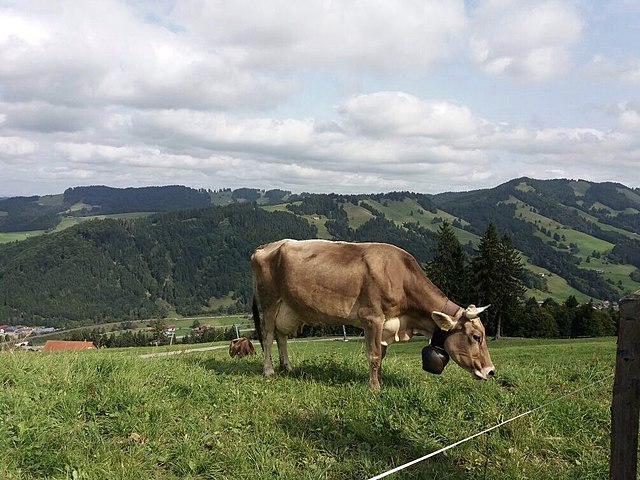
\includegraphics[width=0.45\linewidth]{Bilder/kuh
	}}%
	\bildquelle{\autoref{bild1}: Andrew C, CC BY 2.0, \url{https://w.wiki/33UJ}}
	\bildquelle{\autoref{bild2}: Killarnee, CC BY-SA 4.0, \url{https://w.wiki/33UK}}
	\caption{Verschiedene Bilder in einer Grafik}%
\end{figure}

Zum Zitieren wird der \lstinline|\cite{id}| Befehl verwendet. Dabei können auch Seitenzahlen angegeben werden, z.B. \cite{Haffner2018} oder \cite[S. 15]{Haffner2018}. Der Zitierstil ist in der \path{packages.tex} Datei definiert.

\section{Nützliche Tools}

\begin{itemize}
	\item Mathematische Symbole in Latex: \newline\url{https://detexify.kirelabs.org/classify.html}
	\item Bibliographieverwaltung: z.B. \url{https://www.jabref.org/}
	\item Tabellen: \url{https://www.latex-tables.com/}
\end{itemize}

Generell ist die Verwendung von GIT für die Arbeit zu empfehlen. Durch die Verwendung von Github / Bitbucket / Gitlab lassen sich automatisch Sicherungskopien erzeugen und Versionen verwalten.